% Copyright 2004 by Till Tantau <tantau@users.sourceforge.net>.
%
% In principle, this file can be redistributed and/or modified under
% the terms of the GNU Public License, version 2.
%
% However, this file is supposed to be a template to be modified
% for your own needs. For this reason, if you use this file as a
% template and not specifically distribute it as part of a another
% package/program, I grant the extra permission to freely copy and
% modify this file as you see fit and even to delete this copyright
% notice.


\documentclass{beamer}

\usepackage[spanish]{babel}
\usepackage[utf8]{inputenc}

% There are many different themes available for Beamer. A comprehensive
% list with examples is given here:
% http://deic.uab.es/~iblanes/beamer_gallery/index_by_theme.html
% You can uncomment the themes below if you would like to use a different
% one:
%\usetheme{AnnArbor}
%\usetheme{Antibes}
%\usetheme{Bergen}
%\usetheme{Berkeley}
%\usetheme{Berlin}
%\usetheme{Boadilla}
%\usetheme{boxes}
%\usetheme{CambridgeUS}
%\usetheme{Copenhagen}
%\usetheme{Darmstadt}
%\usetheme{default}
%\usetheme{Frankfurt}
%\usetheme{Goettingen}
%\usetheme{Hannover}
%\usetheme{Ilmenau}
%\usetheme{JuanLesPins}
%\usetheme{Luebeck}
\usetheme{Madrid}
%\usetheme{Malmoe}
%\usetheme{Marburg}
%\usetheme{Montpellier}
%\usetheme{PaloAlto}
%\usetheme{Pittsburgh}
%\usetheme{Rochester}
%\usetheme{Singapore}
%\usetheme{Szeged}
%\usetheme{Warsaw}


\title{Kernel Independant Fast Multipole Method}

% A subtitle is optional and this may be delete

\author{Camilo Valenzuela Carrasco }
% - Give the names in the same order as the appear in the paper.
% - Use the \inst{?} command only if the authors have different
%   affiliation.

\institute[Universidad Técnica Federico Santa Maria] % (optional, but mostly needed)
{Universidad Técnica Federico Santa Maria}
% - Use the \inst command only if there are several affiliations.
% - Keep it simple, no one is interested in your street address.

%\date{}
% - Either use conference name or its abbreviation.
% - Not really informative to the audience, more for people (including
%   yourself) who are reading the slides online

% This is only inserted into the PDF information catalog. Can be left
% out. 

% If you have a file called "university-logo-filename.xxx", where xxx
% is a graphic format that can be processed by latex or pdflatex,
% resp., then you can add a logo as follows:

% \pgfdeclareimage[height=0.5cm]{university-logo}{university-logo-filename}
% \logo{\pgfuseimage{university-logo}}

% Delete this, if you do not want the table of contents to pop up at
% the beginning of each subsection:
\AtBeginSubsection[]
{
  \begin{frame}<beamer>{Outline}
    \tableofcontents[currentsection,currentsubsection]
  \end{frame}
}

% Let's get started
\begin{document}

\begin{frame}
  \titlepage
\end{frame}

% Section and subsections will appear in the presentation overview
% and table of contents.


\begin{frame}{N-Body Problem}
  Dado $N$ densidades ${\phi_i}$ en los puntos ${y_i}$, se desea calcular el potencial ${q_i}$ en un punto target ${x_i}$ inducido por una funcion de Kernel $G$
  \begin{equation}
      q_i = q(x_i)= \sum_{j=1}^N  G(x_i, y_j) \phi(y_j), \ \ \ i = 1 .. N
  \end{equation}
  La implementación directa de esta suma tiene complejidad $O(N^2)$
\end{frame}
\begin{frame}{Fast Multipole Method}
  Fast Multipole Method (FMM) es un algoritmo que busca reducir la complejidad del cálculo de $O(N^2)$ a $O(N)$. Este algoritmo se puede dividir en los siguientes pasos:
  \begin{itemize}
      \item Construcción de un árbol que particiona el dominio.
      \item Calculo de los Monopolos (P2M)
      \item Recursivamente avanzar sobre el árbol (M2M)
      \item Realizar la expansión local (M2L)
      \item Bajar el árbol (L2L)
      \item Evaluar el Far-Field (L2P) y el Near-Field de forma directa.
  \end{itemize}
\end{frame}


\begin{frame}
\begin{center}
 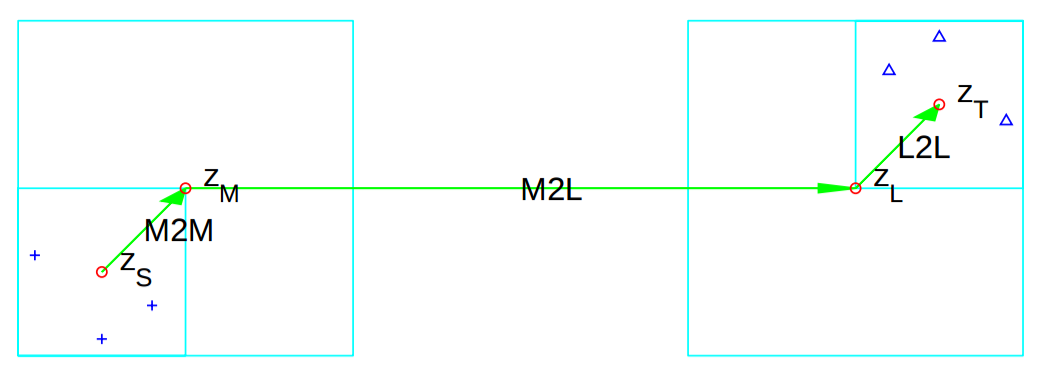
\includegraphics[scale=0.3]{fmm.png}
\end{center}
\end{frame}

\begin{frame}{Problema con FMM}
Requiere un trabajo analítico para crear las expansiones de los sources y targets, además de las transformaciones de M2M, M2L, L2L.
\end{frame}

\begin{frame}{Kernel Independant FMM (KIFMM)}
\begin{itemize}
    \item Dado una funcion de Kernel $G(x,y)$
    \item Se asume que puede ser transformada en un algoritmo FMM. Pero no se conocen sus expansiones ni transformaciones de forma analítica.
    \item Se construye un algoritmo similar a FMM, buscando una complejidad $O(N)$
\end{itemize}
\end{frame}

\begin{frame}{KIFMM (Ying et al.)}
\begin{itemize}
    \item Algoritmo basado en el Adaptive FMM donde la construcción del árbol es similar a Treecode.
    \item Reemplaza las expansiones y transformaciones del FMM por \textit{equivalent density representation}.
\end{itemize}
\end{frame}

\begin{frame}{Equivalent Density - Multipolo}
\begin{itemize}
    \item Dado un conjunto de sources $y_i$ dentro de la caja $B$ queremos calcular 
    $$\displaystyle \sum_{i \in I_s^B} G(x,y_i) \phi_i = q^{B,u}$$
    \item Calculamos esto en un conjunto de puntos en una superficie que encierra $B$ (\textit{check surface}).
    Por lo que la suma anterior se tiene que cumplir para todo $x \in x^{B,u}$.
    \item Elegimos ahora una superficie entre la caja y nuestra \textit{check surface} que llamaremos \textit{equivalent surface}.
    \item Estas superficies son elegidas tal que cumplan 
    $$\int_{y^{B,u}}  G(x,y_i) \phi^{B,u}(y) dy= \sum_{i\in I^{B}_s} G(x,y_i) \phi_i = q^{B,u} \ \ para \ cualquier \ x \in x^{B,u} $$
\end{itemize}

\end{frame}
\begin{frame}{Equivalent Density - Local}
 Similar al Monopolo elegimos una \textit{check surface} y una \textit{equivalent surface} la diferencia es que la \textit{check surface} queda entre la caja y la \textit{equivalent surface}.
 
 Al igual que el caso anterior se tiene que cumplir que 
  $$\int_{y^{B,d}}  G(x,y_i) \phi^{B,d} dy = \sum_{i\in I^{B}_s} G(x,y_i) \phi_i = q^{B,d} $$

\end{frame}
\begin{frame}
 \begin{center}
 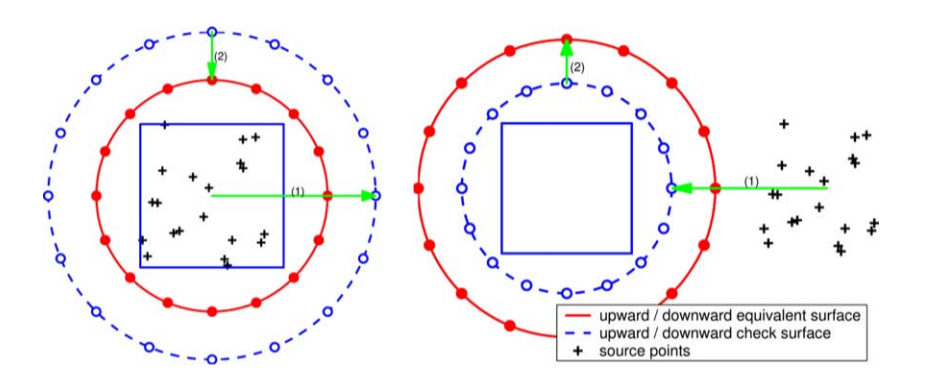
\includegraphics[scale=0.4]{densities.png}
 \end{center}
\end{frame}
\begin{frame}{Transformaciones}
\begin{itemize}
    \item M2M: El potencial de la caja padre tiene que ser igual al potencial equivalente del hijo
    $$ \int_{y^{B,u}} G(x,y) \phi^{B,u}(y) dy = \int_{y^{A,u}} G(x,y) \phi^{A,u}(y) dy$$
    \item M2L: El potencial de la caja source tiene que ser igual al potencial de la caja target.
    $$ \int_{y^{B,u}} G(x,y) \phi^{B,u}(y) dy = \int_{y^{A,d}} G(x,y) \phi^{A,d}(y) dy$$
    \item L2L: Igual que en M2M pero en caso local
    $$ \int_{y^{B,d}} G(x,y) \phi^{B,d}(y) dy = \int_{y^{A,d}} G(x,y) \phi^{A,d}(y) dy$$
\end{itemize}
\end{frame}

\begin{frame}
 \begin{center}
 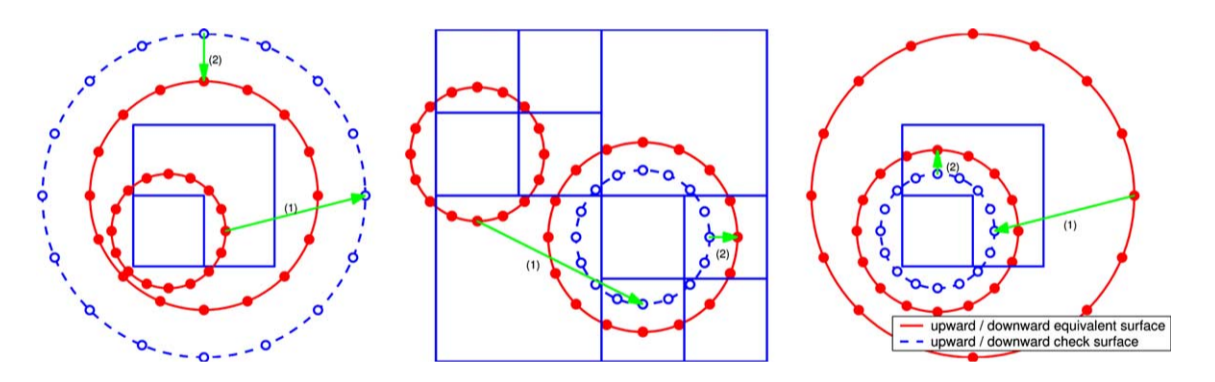
\includegraphics[scale=0.27]{transformation.png}
 \end{center}
\end{frame}
\begin{frame}{Resolviendo las ecuaciones}
Luego de discretizar las ecuaciones se pueden representar de forma matricial de la forma
$$ K \phi = q$$
Para resolverlas de forma estable se ocupa
$$\phi = \left( \alpha I  + K^*K \right)^{-1}K^*q$$
\end{frame}

\begin{frame}{Algoritmo}
\begin{enumerate}
    \item Crear árbol del dominio
    \item Por cada hoja $B$ calculamos
    \begin{itemize}
        \item evalaur $q^{B,u}$ en los puntox $x^{B,u}$ usando $\{\phi_i, i \in I_s^B\}$
        \item resolver la ecuación integral para obtener $\phi^{B,u}$ para que sea igual a $q^{B,u}$
    \end{itemize}
    \item Se realiza M2M
    \begin{itemize}
        \item calcular $q^{B,u}$ utilizando los $\phi^{C,u}$ de los hijos C de la caja B.
        \item resolver la eucación para obtener $\phi^{B,u}$
    \end{itemize}
    \item Se realiza M2L
    \item Se baja por el árbol con L2L.
    \item Evaluamos el farfield con L2P y el nearfield con evaluación directa.

    \item Llevar las densidades equivalentes a los targets (M2L).
\end{enumerate}
\end{frame}

\begin{frame}{Conclusiones}
\begin{itemize}
    \item Utilizar FMM con un nuevo kernel necesita un gran trabajo analítico.
    \item Existen algunos FMM independientes del Kernel.
    \item Los KIFMM no siempre obtienen la misma complejidad o precisión que FMM.
\end{itemize}
\end{frame}
\end{document}


